%!TEX root = ../../prj4projektdokumentation.tex
% SKAL STÅ I TOPPEN AF ALLE FILER FOR AT MASTER-filen KOMPILERES 

\section{Allokeringsdiagram}
På figur \ref{fig:Allokering} ses allokeringsdiagram for spændningsregulatoren. Diagrammet er lavet for at danne overblik over softwaren, derfor er analog moduler undladt. Diagrammet viser hvilke platforme de logiske blokke skal laves på, og hvordan kommunikationen er mellem blokkene.

\begin{enumerate}
	\item Brugergrænsefladen allokeres på en HMI skærm.
	\item Kontrolmodulet allokeres på en PLC.
	\item Kommunikationsmodulet allokeres på en Arduino.
	\item Måleenhederne allokeres på PSoCs.
\end{enumerate}   
Kommunikationen mellem blokkene er allokeret på tre forskellige protokoller, se Kapitel \ref{ch:KomProtokol} for uddybning af disse.
\begin{enumerate}
	\item Mellem HMI og PLC anvendes Siemens standard PROFIBUS
	\item Mellem PLC og Arduino anvendes en TCP-protokol
	\item Mellem Arduino og PSOC anvendes en UART-protokol
\end{enumerate}

\begin{figure}[htbp] % (alternativt [H])
	\centering
	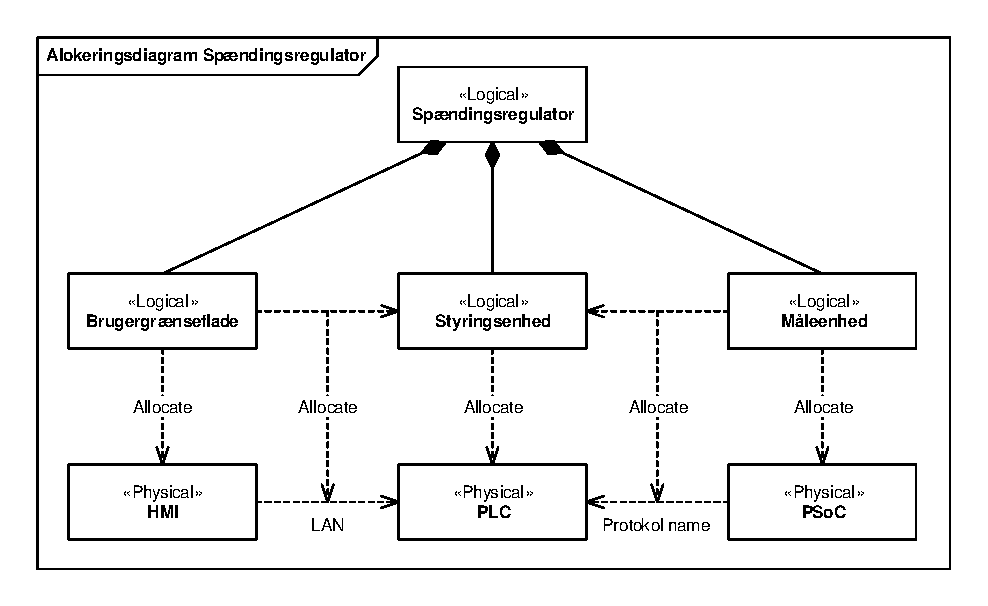
\includegraphics[width=0.9\textwidth]{Figure/Allokering}
	\caption{Allokeringsdiagram for spændingsregulator}
	\label{fig:Allokering}
\end{figure}

\newpage